\documentclass[11pt]{report}
\clubpenalty=10000
\widowpenalty=10000

% It is handy to define new commands for text that occurs frequently (see Discussion)
\newcommand{\MT}{^{\mathrm{MT}}}
\newcommand{\ga}{\gtrsim}
\newcommand{\Lpot}{(L+1)^2}
\newcommand{\WS}{^{\mathrm{WS}}}

%--Format the section headers

\usepackage{amsmath}
\usepackage{amsfonts}
\usepackage{amssymb}
\usepackage{wasysym}
\usepackage{graphicx}
\usepackage{pslatex}
\usepackage{lscape}
\usepackage[T1]{fontenc}
\usepackage[latin1]{inputenc}
\usepackage{longtable}
 \setlength{\LTcapwidth}{5.5 in}
\usepackage{chapterbib}
\usepackage{fancyhdr} % for better header layout
\usepackage{eucal}
\usepackage[english]{babel}
\usepackage[usenames, dvipsnames]{color}
\usepackage[perpage]{footmisc}
\usepackage[round, sort, numbers, authoryear]{natbib}
%\usepackage{multicol} % for pages with multiple text columns, e.g. References
\setlength{\columnsep}{20pt} % space between columns; default 10pt quite narrow
\usepackage[nottoc]{tocbibind} % correct page numbers for bib in TOC, nottoc suppresses an entry for TOC itself
\usepackage{geometry}
\usepackage{setspace}
\usepackage{url}
\usepackage{lastpage}
% FJS Changed this... I didn't like the numbering or the
% indentation... so I introduced a fake chapter Main Text. 
\setcounter{secnumdepth}{0}
\setcounter{tocdepth}{5}

%--set the page formatting--
\geometry{hmargin={1.6in,1.1in},vmargin={1.5in,1.2in}}
\doublespacing

\begin{document}
%--front matter needs roman pagination--
\pagenumbering{roman}

%--Title Page--
\thispagestyle{empty}
  \begin{center}
    \textsc{\LARGE Evaluating Forecasting Methods for\\ Precipitation from Weather Data on top of Guyot Hall } %Fill in your information
  \end{center}
  \vspace{.6in}
  \begin{center}
      Tyrone Zhang
  \end{center}
  \vspace{.6in}
  \begin{center}
    \textsc{A Senior Thesis \\ %Fill in your information
    Presented to the Faculty \\
    of Princeton University \\
    in Candidacy for the Degree \\
    of Bachelor of Arts}
  \end{center}
  \vspace{.3in}
  \begin{center}
    \textsc{Recommended for Acceptance \\
    by the \\Department of  Geosciences \\}
    Adviser: Frederik J.~Simons
  \end{center}
  \vspace{.3in}
  \begin{center}
  \today
  \end{center}
  
  \clearpage


%--Copyright Page--
\thispagestyle{empty}
\vspace*{3in}
\begin{center}
\emph{This paper represents my own work in accordance with University regulations,} \\
Your Signature %%Sign here
\end{center}
\clearpage

%--Abstract--  
\addcontentsline{toc}{chapter}{Abstract}
\begin{center}
\Large \textbf{Abstract}
\end{center}
 
% Senior thesis or Junior Project Abstract -----------------------------------------------------

Princeton's climate has four seasons, with strong temperature
variations, and precipitation occurring throughout the
year. Statistically, precipitation event sequences can be
characterized as drawn from exponential distributions in the three
variables the precipitation event \textit{duration}, \textit{intensity} 
(the total precipitation divided by the duration), and the non-precipitation 
\textit{duration}. The shortest and least intense precipitation events 
are the most frequent. Analyzing the precipitation measured from 2017 
to the present day by a Vaisala WXT530 weather station located on the 
roof of Guyot Hall, I first summarize the data in terms
of exponential distributions and their parameters, by season and by
year. Subsequently, I evaluate the skill in predicting the arrival,
duration and intensity of precipitation events solely based on this
local ``climatology'', before including other variables logged by the
weather station. Predicting precipitation events using this climatology
yielded 2-3 \% precipitation accuracy. Thus, we proceeded to use linear
regression and decision trees regression to improve the precipitation
accuracy. Linear regression yielded 4.7 \%, while decision tree yielded 
11.9\%. Then neural networks were used in the form of LSTM, where we had 
hourly and minute inputs. The hourly input
resulted in 9.9\%, while the minute inputs resulted in 16.8\%. With each new model, 
we are able to see improvements in the accuracy of
predicting precipitation. However, there are further improvements that can be 
made with many pathways forward to improve the precipitation accuracy.  

 \clearpage

%--Acknowledgements--  
\addcontentsline{toc}{chapter}{Acknowledgements}
\begin{center}
\Large \textbf{Acknowledgements}
\end{center}

% Senior thesis or Junior Project Acknowledgements  -----------------------------------------------------

%Delete the text below and write your acknowledgements
I would like to acknowledge my senior thesis advisor Frederik J. Simons for giving me constant feedback on my work as well as providing me with the data that he is collecting on top of Guyot Hall. 
\clearpage

%--Table of Contents--  
\thispagestyle{empty}
\tableofcontents
\clearpage

\listoffigures
\listoftables
\clearpage

%--Set up fancy header-- 
\fancyhead{}
\fancyfoot{}
\pagestyle{fancyplain}
\rhead{\fancyplain{\thepage}{\noindent \textsc{\rightmark} \hfill \thepage~of~\pageref{LastPage}}}
\rfoot{\hrule \today \hfill Your Name}
\pagenumbering{arabic}

%--Reset the page numbers and set them to arabic-- 
{\newpage\renewcommand{\thepage}{\arabic{page}}\setcounter{page}{1}}

%--Have sections but use chapter counters
\addcontentsline{toc}{chapter}{Main Text}

\section{Introduction \label{sec:introduction}}

The introduction should convey the purpose and scope of your study. The introduction also is where you include relevant background text and figures that give the reader the necessary context to understand the importance and meaning of your study. For example, the introduction might contain a map (Fig. \ref{fig:map}) depicting sample locations.

\begin{figure}[h!]
\centering
\includegraphics[width=0.85\textwidth]{Figures/example-map.pdf}
\caption[Short title for this figure that fits on a line]{\small{(a)~Simplified geological map \citep[adapted from][]{Preiss2002a}) of the study area within the Adelaide Rift Complex (ARC). Locations of measured stratigraphic sections are denoted by red circles and labeled with numbered squares. (b)~Schematic NW-SE stratigraphic cross-section of the Adelaide Rift Complex, highlighting the rift-to-drift transition and major sequence boundaries and U-Pb zircon ages. The $\delta^{13}$C$_{carb}$ profile \citep[adapted from][]{Halverson2005a} is time-aligned with the right-hand edge of the stratigraphic cross-section.}} 
\label{fig:map}
\end{figure}

\section{Methods \label{sec:methods}}
The methods section should describe how you conducted field work, how you collected samples, how you designed lab work, what analytical methods you employed, etc. For example, if you collected GPS data, you would describe what type of electronics you used, how you designed your sampling, and how you measured the accuracy of individual measurements. You would accompany this information with a table or graph depicting, for example, the reproducibility of GPS measurements from identical physical locations at different times.

As another example, if you were modeling the strontium cycle in the ocean with the following mass balance equations, you could explain where these equations come from, and include Table (\ref{tab:sr}) to collect information about the model variables.
\vspace{-10pt}
\begin{eqnarray}
\frac{dMg}{dt} &=& W_{Mg-carb} + W_{Mg-sil} - H_{Mg-clays} - P_{Mg-carb} \\
\frac{dCa}{dt} &=& W_{Ca-carb} + W_{Ca-sil} + H_{Ca-basalt} - P_{Ca-carb} \\
\frac{d^{n}Sr}{dt} &=& W_{^{n}Sr-carb} + W_{^{n}Sr-sil} + H_{^{n}Sr-basalt} - P_{^{n}Sr-carb},
\end{eqnarray}
\vspace{-20pt}
\linespread{1}
\tabcolsep 2.5pt 
\begin{table}[h!]
\centering
$ $\\
\footnotesize{}
\begin{tabular}{c|c|c|c}
Model Variable & & & \\
\hline
weathering & & hydrothermal & \\
\hline
$W_{Mg-carb}$ & 2.0$\times$10$^{12}$ mol/yr$^{1}$ & $k$ & 3.75$\times$10$^{13}$ kg H$_2$O/yr \\
$W_{Ca-carb}$ & 10.5$\times$10$^{12}$ mol/yr$^{1}$ & $H_{Mg-clays}$ & $k \cdot [Mg]$ \\
$W_{total_{Sr-carb}}$ & 1.1$\times$10$^{10}$ mol/yr$^{2}$ & $H_{total_{Sr-basalt}}$ & $\alpha_{Sr/Ca} \cdot H_{Ca-basalt}$ \\
$W_{Mg-sil}$ & 4.0$\times$10$^{12}$ mol/yr$^{1}$ & $\alpha_{Mg/Ca}$ & 1$^4$ \\
$W_{Ca-sil}$ & 4.5$\times$10$^{12}$ mol/yr$^{1}$ & $\alpha_{Sr/Ca}$ & 0.0012$^{5}$ \\
$W_{total_{Sr-sil}}$ & 0.8$\times$10$^{10}$ mol yr$^{2}$ & & \\
& & & \\
$^{87}$Sr/$^{86}$Sr & & precipitation & \\
\hline
$W_{^{87/86}Sr-sil}$ & 0.7200$^2$ & $P_{Ca-carb}$ & 8.75$\times$10$^{12}$ mol/yr$^{6}$ \\
$W_{^{87/86}Sr-carb}$ & 0.7075$^2$ & $P_{Mg-carb}$ & 1.6$\times$10$^{12}$ mol/yr$^{7}$ \\
$H_{^{87/86}Sr-basalt}$ & 0.7030$^2$ & $P_{total_{Sr-carb}}$ & $(Sr/Ca)_{seawater} \cdot K_{Sr} \cdot P_{Ca-carb}$ \\
 & & $K_{Sr}$ & 0.2$^8$ \\
\end{tabular}
$ $\\
\caption[Short title for this table that fits on a line]{\small{Variables used in the numerical model of Mg, Ca, and Sr. $^1$\citet{Meybeck2003a}; $^2$\citet{Allegre2010a}; $^3$flux of H$_2$O in hydrothermal systems assuming 100\% of the heat flux at 350$^{\circ}$C \citep{Elderfield1996a}; $^4$assumes 1:1 stoichiometry between Mg uptake and Ca release during basalt alteration; $^5$calculated assuming 200~ppm Sr and 10~wt\% CaO; $^6$calculated assuming carbonate minerals are the only alkalinity sink; $^7$estimated from the long-term rate of dolomitization \citep{Wilkinson1989a}; $^8$homogeneous distribution coefficient for Sr in calcite \citep{Mucci1983a}. \label{tab:sr}}}
\end{table}

\section{Results \label{sec:results}}
This section will contain the bulk of your tables and figures, describing and illustrating the data you collected for your project. Do not interpret your data in the Results section. For example, let's say you collected information about the minimum ejecta thickness around a $\sim$2~km diameter bolide impact crater in India. You could collect those results in a figure like Fig. \ref{fig:ejecta}. However, you would avoid discussing the significance and meaning of these results until the Discussion section.

\begin{figure}[h!]
  \centering 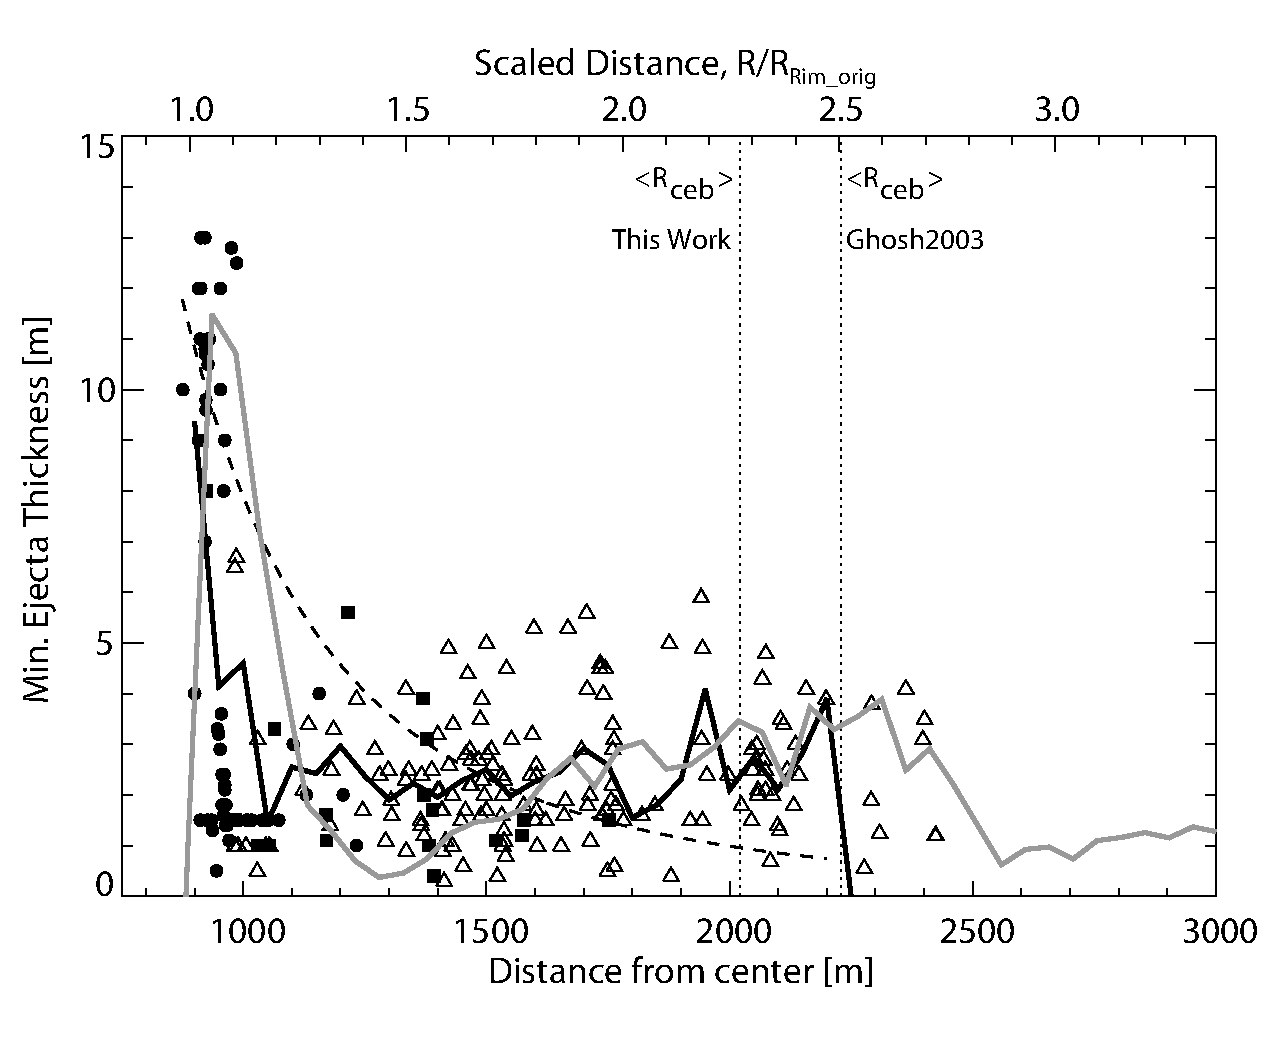
\includegraphics[width=5in]{Figures/example-results.pdf}
\caption[Short title for this figure that fits on a line]{\small{Minimum ejecta thickness measurements (circles-rim fold; squares-large blocks; triangles-small clasts at Lonar Crater, India. Average Lonar ejecta thickness profile (solid line) is compared to a ballistic ejecta thickness from experimental craters \cite[dashed line][]{Mcgetchin73} and the topographic profile for a typical fresh Martian crater \citep[grey line, scaled to Earth][]{StewartValiant06}. $R_{ceb}$ denotes the average extent of the continuous ejecta blanket (vertical dotted lines).  Note the accumulation of ejecta amounting to \textasciitilde{}5 times ballistic predictions at the distal edge of continuous ejecta blanket. \label{fig:ejecta}}}
\end{figure}

\section{Discussion \label{sec:discussion}}
The Discussion section is where you have the chance to interpret the results you just reported on. Additional figures to illustrate your interpretations are useful. For example, you might compile your data with data from other sources  to challenge existing hypotheses or generate new big-picture ideas.

So at this point we might sum up the main findings with a summary figure, for instance, as follows from \cite{Dahlen+2008}. Fig.~\ref{MTvarfig2} shows the large-$l$ variance ratio $(\sigma_{\infty}^2)\MT$ plotted versus the bandwidths $0\leq L\leq 20$ for single polar caps of various radii $0^{\circ}\leq\Theta\leq 180^{\circ}$ and double polar caps of various radii $0^{\circ}\leq\Theta\leq 90^{\circ}$. In the degenerate case $L=0$, bandlimited `multitaper' estimation is tantamount to whole-sphere estimation so $(\sigma_{\infty}^2)\MT=1$ regardless of the `cap' size $\Theta$. Indeed, in that case, the estimate is unbiased, $M_{ll'}=\delta_{ll'}$, and at $L=0$, the single possible taper is a constant over the entire sphere. For sufficiently large regions ($\Theta\ga 30^{\circ}$ for a single cap and $\Theta\ga 15^{\circ}$ for a double cap) the large-$l$ variance ratio is a monotonically decreasing function of the bandwidth $L$; for smaller regions the ratio attains a maximum value $(\sigma_{\infty}^2)\MT>1$ before decreasing. The grey curves are isolines of fixed Shannon number $K=(A/4\pi)\Lpot$; it is noteworthy that the $K=1$ isoline passes roughly through the maxima of $(\sigma_{\infty}^2)\MT$, so that for $K\geq 2$--3 the variance ratio is a decreasing function of the bandwidth $L$ regardless of the cap size.  Since $K$ is the number of retained tapers, it will always be greater than 2--3 in a realistic multitaper analysis. For large Shannon numbers, above $K\approx 10$, the dependence upon the bandwidth $L$ and area $A$ for both a single or double cap can be approximated by the empirical relation $(\sigma_{\infty}^2)\MT\approx (4\pi/A)^{0.88}/(2L+1)$.  In particular, if $A=4\pi$, the large-$l$ variance ratio is to a very good approximation equal to one divided by the number of adjacent degrees $l-L\leq l'\leq l+L$ that are averaged over by the coupling matrix $M_{ll'}$. As noted in Section~\ref{sec:methods}, a whole-sphere multitaper estimate $\hat{S}_l\MT$ can be regarded as a weighted linear combination of whole-sphere estimates of the form $\sum_{l'}M_{ll'}\hat{S}_{l'}\WS$, so the variance is reduced by the number of independent random variates $\hat{S}_{l-L}\WS,\ldots,\hat{S}_l\WS, \ldots, \hat{S}_{l+L}\WS$ that contribute to the estimate.  For smaller regions of area $A\approx 4\pi$ the whole-sphere variance ratio $1/(2L+1)$ is empirically found to be increased by a factor $(4\pi/A)^{0.88}$. In fact, it is very reasonable to approximate the nearly-whole-sphere variance ratio at large Shannon numbers by $(\sigma_l^2)\MT\approx (4\pi/A)^{0.88}(\sigma_l^2)\MT_{A=4\pi}$ for all spherical harmonic degrees $0\leq l\leq\infty$.

\begin{figure}
\centering 
\rotatebox{0}{
\includegraphics[width=1\textwidth]{Figures/example-discussion.pdf}
} 
\caption[Variance ratio of multitaper estimates]{Variation of the large-$l$ multitaper variance ratio $(\sigma_{\infty}^2)\MT$ with bandwidth $0\leq L\leq 20$ for single polar caps of radii $\Theta=0^{\circ},10^{\circ},20^{\circ}, 30^{\circ},40^{\circ},50^{\circ},70^{\circ},100^{\circ},180^{\circ}$ (left) and double polar caps of common radii $\Theta=0^{\circ}, 5^{\circ}, 10^{\circ}, 20^{\circ},30^{\circ},40^{\circ},60^{\circ},90^{\circ}$ (right). Ranges of the Shannon number $K=(A/4\pi)\Lpot$ are distinguished by different symbols: open circles $0\leq K\leq 1$, closed circles $1\leq K\leq 10$, open squares $10\leq K\leq 100$, closed squares $K\geq 100$. Grey curves labeled \mbox{$K=1,10,100$} are Shannon number  isolines. Axes are logarithmic to illustrate the $1/(2L+1)$ bandwidth scaling above $K\approx 10$. \label{MTvarfig2}}
\end{figure}

\section{Conclusions \label{sec:conclusions}}
Unlike the Results section (page~\pageref{sec:results}), this section should be a clear statement of the major conclusions you have drawn from your work. The conclusions should follow clearly from the Results and Discussion sections.

%--References
\small
\renewcommand{\bibsep}{0em}

\renewcommand{\bibname}{References}
\bibliographystyle{Latex/gji}
\bibliography{refs}

\end{document}
